\documentclass{beamer}
\usecolortheme{beaver}
\usetheme{CambridgeUS}
\usepackage[export]{adjustbox}

\begin{document}
\title[Hair Rendering]{Hair Rendering:\\ Importance
Sampling of Dual Scattering
Approximation}
\author[J. Lemein]{Jeffrey Lemein\\\small Supervisor: Prof. Remco Veltkamp \\ \hspace{18mm}}
\institute[Master Thesis]{Department of Information and Computing Sciences\\Utrecht University}
\date{\today}

\begin{frame}
\titlepage
\end{frame}

\begin{frame}
\frametitle{Goal of thesis}
\centering
\textit{"To evaluate whether multiple importance sampling (MIS) the dualscattering method leads to a significant reduction of variance in the rendered results".}

\end{frame}


  \begin{frame}
    \frametitle{Background}
	\framesubtitle{Rendering hair}
	
	Important for variety of industries
	\begin{itemize}
	\item Animation movie industry: to render realistic hairs in a physically accurate way.
	\item Game industry: enhance realism and visual effects.
	\item Clothes manufacturing industry: to render custom fabrics and to compare appearance in different lighting conditions.
	\item Hair styling: render hair styling products applied to the hair.
	\end{itemize}
  \end{frame}
  
  \begin{frame}
    \frametitle{Rendering hair}
	\framesubtitle{Hair fiber representation}
	Explicit representation vs. Implicit representation
	
	\begin{itemize}
	\item Explicit representation represents each fiber by geometric primitives (e.g. triangles)
	\item Implicit representation represents fiber
	\end{itemize}
	
	There are a couple of ways to represent hair fibers:
	\begin{itemize}
	\item Camera-facing triangle strips
	\item Cylindrical primitives (used in thesis)
	\item Trigonal prisms
	\item Ribbons
	\end{itemize}
	

  \end{frame}
  
  \begin{frame}
    \frametitle{Rendering hair}
	\framesubtitle{Rendering challenges}
	
	Human hair consists of over hundreds of thousands of hair strands.
	Leads to rendering challenges:
	\begin{itemize}
	\item Memory consumption: to store all fibers in memory.
	\item Time: rendering realistic scattering effects requires tracing many samples through the hair volume.
	\item Aliasing: Hair fibers are very thin, requiring additional samples to be drawn to prevent aliasing.
	\end{itemize}
	

  \end{frame}
  
  % end Rendering hair
  
  \begin{frame}
    \frametitle{Mathematical notation}
	\framesubtitle{Radiometry}
	\begin{itemize}
	\item Power (Watts): energy in Joules per second.
	\item Radiant intensity (steradians): power divided by the solid angle.
	\item Irradiance (Watts per $m^2$): power per unit area.
	\item Radiance : Irradiance per solid angle, where solid angle goes to zero (becoming a ray instead of a cone).
	\end{itemize}
  \end{frame}
  
  \begin{frame}
    \frametitle{Mathematical notation}
	\framesubtitle{Scattering equations}
	
	Scattering is represented by a bidirectional reflection distribution function (BRDF):
	
	\begin{equation}
	f_r(p, \omega_o, \omega_i) = \frac{dL_o(p, \omega_o)}{dE(p, \omega_i)} = \frac{dL_o(p, \omega_o)}{L_i(p, \omega_i) \cos \theta_i d\omega_i}
	\end{equation}
	
	The BRDF is the fraction of outgoing radiance in direction $\omega_o$ related to the incident irradiance from direction $\omega_i$.

  \end{frame}
  
  
  \begin{frame}
    \frametitle{Mathematical notation}
	\framesubtitle{Coordinates axes for hair fibers}

\includegraphics[width=0.5\textwidth,center]{../thesis/images/axes.png}

\begin{itemize}
\item Coordinate axis are represented using $uvw$ axes, with $u$ pointing from base to tip of hair strand and $vw$ forms the orthogonal plane.
	
\item Longitudinal angles $\theta$ are with respect to $u$, where 0 degrees is perpendicular to the fiber, -90 towards base, and 90 towards tip.
	
\item Azimuthal angles $\phi$ are formed with respect to the orthogonal plane.
	
	\item $\omega_i = (\theta_i, \phi_i)$ incident direction, $\omega_o = (\theta_o, \phi_o)$ outgoing direction.
\end{itemize}	
	
	\end{frame}
  
\begin{frame}
    \frametitle{Mathematical notation}
	\framesubtitle{Bidirectional curve scattering distribution function (BCSDF)}
	
	\begin{itemize}
	\item Hair fibers are rendered implicitly by 3D curves.
	\item Curves have no surface area. They have a length, requiring a change to the BRDF formulation.
	\end{itemize}
	
	\begin{equation}
	S_r(\omega_o, \omega_i) = \frac{dL_o(\omega_o)}{dE_i(\omega_i)} = \frac{dL_o(\omega_o)}{DL_i(\omega_i) \cos \theta_i d\omega_i}
	\end{equation}
	
	\begin{equation}
	L_o(\omega_o) = D \int S(\omega_i, \omega_o) L_i(\omega_i) \cos \theta_i d\omega_i
	\end{equation}

  \end{frame}  
  
  
% end mathematical notation  
  
  \begin{frame}
    \frametitle{Monte-Carlo integration}
    
    Let's say we want to integrate $f(x)$ which is a  1D formula from $a$ to $b$.
    
    \begin{equation}
    \int_a^b f(x) dx
    \end{equation}
    
	This can be evaluated by drawing $N$ uniform samples for $X_i \in [a, b]$.
    
    \begin{equation}
    F_N = \frac{b-a}{N} \sum^N_{i=1} f(X_i)
    \end{equation}
    
    The Monte-Carlo estimator says that the expected value $E[F_N]$ is equal to the integral.
    
    Possible to integrate any definite higher dimensional integrals.
    
  \end{frame}
  
  \begin{frame}
    \frametitle{Importance sampling}
    
    \begin{itemize}
    \item Reduces noise faster by sampling high-value contributions.
    
    \item The estimator can be rewritten by taking into consideration the probability density function $p(X_i)$
    
    \item Samples need to be generated from $p(x)$, by processes such as the inversion method or rejection method.
    
    \end{itemize}
    
     \begin{equation}
    F_N = \frac{1}{N} \sum^N_{i=1} \frac{f(X_i)}{p(X_i)}
    \end{equation}
    
  \end{frame}
  
    
  \begin{frame}
    \frametitle{Multiple importance sampling}
    
    \begin{itemize}
    \item Scattering distributions cannot always be represented by closed formulas, or be inverted at all.
    
    \item A solution is to match the scattering distribution with multiple simple functions $f(x)$ and $g(x)$
    \end{itemize}
    
        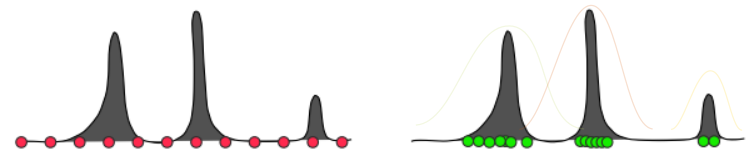
\includegraphics[width=0.8\textwidth,center]{importance_sampling_px.png}
    
    \begin{equation}
\frac{1}{n_f} \sum_{i=1}^{n_f} \frac{f(X_i)g(X_i) w_f(X_i)}{p_f(X_i)} + 
\frac{1}{n_g} \sum_{j=1}^{n_g} \frac{f(Y_j)g(Y_j) w_g(Y_j)}{p_g(Y_j)} 
\end{equation}

\begin{equation}
w_s(x) = \frac{n_sp_s(x)}{\sum_i n_i p_i(x)}
\end{equation}

    
  \end{frame}

	% end Importance sampling
  
  \begin{frame}
    \frametitle{Related work}
	\framesubtitle{Structure of hair}
	
	\begin{itemize}
	\item Hair fibers do have cuticle scales tilted by approximately 3 degrees toward the root.
	\item The core of the fiber (medulla and cortex) consist of pigment which absorbs specific wavelengths in the light.
	\end{itemize}
	
	\begin{figure}
	\includegraphics[scale=0.3]{../thesis/images/hair_structure.jpeg}
	\includegraphics[scale=0.25]{../thesis/hair-core.png}
	\end{figure}
  \end{frame}
  
  
  \begin{frame}
    \frametitle{Related work}
    \framesubtitle{Measured scattering data}
    Single fiber scattering model that models three visible scattering components:
    
    \begin{figure}
    \centering
    \includegraphics[scale=0.25]{../thesis/images/longitudinal_response.jpeg}
    \end{figure}
  \end{frame}
  
    \begin{frame}
    \frametitle{Related work}
    \framesubtitle{Marschner model}
    Marschner et al. (2003) proposed a single fiber scattering model for three visible scattering components.
    \begin{itemize}
    \centering
    \item[R] reflection,
    \item[TT] double transmission,
    \item[TRT] transmission, reflection, transmission
    \end{itemize}
    
    \includegraphics[width=0.3\textwidth, center]{../thesis/images/female_marschner.jpeg}
    
  \end{frame}
  
  \begin{frame}
  \frametitle{Related work}
  \framesubtitle{Marschner model: longitudinal scattering M}
  The Marschner model scattering equation can be written as:
  
  \begin{equation}
  S(\omega_i, \omega_o) = \sum_p M_p(\theta_i, \theta_o) N_p(\eta(\theta_d); \phi_i, \phi_o) / \cos^2 \theta_d
  \end{equation}
  
  \begin{columns}[onlytextwidth]
    \begin{column}{.5\textwidth}
    	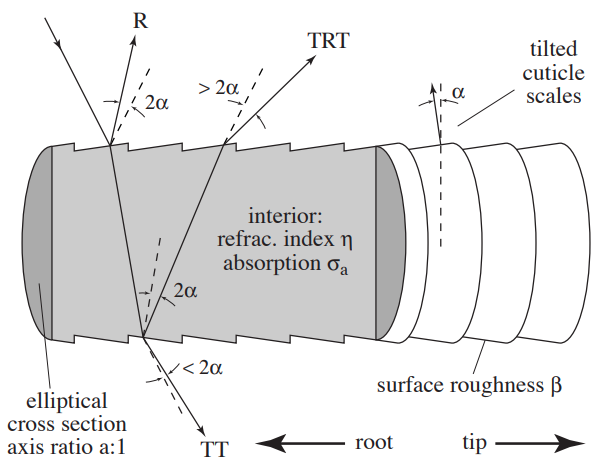
\includegraphics[width=\textwidth,center]{../thesis/images/marschner_model_longitudinal.png}
    \end{column}
    \begin{column}{.5\textwidth}
    \centering
    \begin{equation}
  M_p(\theta_h) = g(\beta_p; \theta_h-\alpha_p)
  \end{equation}  
  \begin{itemize}
  \item $p$ is the scattering mode with $p \in {R, TT, TRT}$
  \item where $\theta_h$ is the half angle between $\theta_i$ and $\theta_o$
  \end{itemize}
    \end{column}
    \end{columns}
   
  
  
  \end{frame}
  
  \begin{frame}
  \frametitle{Related work}
  \framesubtitle{Marschner model: azimuthal scattering N}
  
  \begin{columns}[onlytextwidth]
    \begin{column}{.50\textwidth}
    	\includegraphics[width=\textwidth,center]{../thesis/circularcross.png}
    \end{column}

    \begin{column}{.50\textwidth}
    \begin{align*}
  N(\phi) &= \sum_p N_p(p, \phi) \\
  N_p(\theta_h) &= \sum_r A(p, h) \mid 2 \frac{d\phi}{dh}(p, h)\mid
  \end{align*}
   \begin{itemize}
  \item $r$ is the number of roots $h$.
  \item where $\eta$ is the index of refraction.
  \item $A$ is the absorption coefficient
  \end{itemize}
    \end{column}
    \end{columns}
  
 
  \end{frame}
  
  \begin{frame}
    \frametitle{Related work}
    \framesubtitle{Dualscattering Approximation}

\begin{itemize}
\item Marschner model deals with rendering a single fiber.
	
\item Path-tracing have to be performed to render globally illuminated hair volumes.

\begin{itemize}
\item Very costly, takes a lot of time.
\item Requires a lot of samples to reduce noise.
\end{itemize}
\end{itemize}

Dualscattering approximation by Zinke et al.(2008) proposes a dual approach to overcome the extensive path tracing.

  \end{frame}  
  
  \begin{frame}
    \frametitle{Related work}
    \framesubtitle{Dualscattering approximation}
    Dualscattering approximation breaks the scattering computation up into two components
    \begin{itemize}
    \item Global scattering $\Psi^G$: Computes the irradiance arriving at a point $x$ in the hair volume.
        \item Local scattering $\Psi^L$: Accounts for the multiple scattering within the neighborhood of point $x$
    \end{itemize}
  \end{frame}
  
  
    \begin{frame}
    \frametitle{Related work}
    \framesubtitle{Dualscattering: global scattering}
    
    Global scattering $\Psi^G$ is computed by taking into account:
    
    \begin{itemize}
    \item Transmittance $T_f$ through the volume from direction $\omega_d$
    \item Spread $S_f$ when scattering through hair strands.
    \end{itemize}
    
    \begin{equation}
\Psi^G(x, \omega_d, \omega_i) \approx T_f(x, \omega_d)\,S_f(x, \omega_d, \omega_i)
\end{equation}

\begin{columns}
\begin{column}{0.4\textwidth}

\begin{align*}
T_f(x, \omega_d) &= d_f \cdot \prod_{k=1}^{n} a_f(\theta_d^k) \approx d_f \cdot a_f(\theta_d)^n \\
S_f(x, \omega_d, \omega_i) &= \frac{g(\theta_d + \theta_i, \sigma_f^2)}{\pi \cos \theta_d}  \\
\sigma_f^2(x, \omega_d) &= \sum_{k=1}^{n} \beta_f^2(\theta_d^k) \approx n \cdot \beta_f^2(\theta_d) \\
\end{align*}

\end{column}
\begin{column}{0.4\textwidth}
   \includegraphics[width=0.85\textwidth, right]{../thesis/relatedwork/dualscattering_df.png}
   \end{column}
   \end{columns}
  \end{frame}
  
   \begin{frame}
    \frametitle{Related work}
    \framesubtitle{Dualscattering: local scattering}

\begin{itemize}    
\item Local scattering $\Psi^L$ deals with local neighborhood by rendering them using the Marschner model $f_s$.
\item Forward scattering events are dealt with by global scatter component.
\item Local scattering needs to deal with at least one backscatter event
\end{itemize}

\begin{equation}
\Psi^L(x, \omega_d, \omega_i) f_s(\omega_i,\omega_o) \approx d_b \cdot f_{back}(\omega_i, \omega_o)
\end{equation}

\begin{equation}
f_{back}(\omega_i, \omega_o) = \frac{2}{\cos \theta_d} A_b(\theta_d) \cdot S_b(\omega_i, \omega_o)
\end{equation}

where $A_b$ is the average backscattering attenuation and $S_b$ the average backscattering spread.
    
  \end{frame}
  
  \begin{frame}
    \frametitle{Approach}
	Goal of thesis:
	
	\begin{center}
	\textit{"To evaluate whether multiple importance sampling (MIS) the dualscattering method leads to a significant reduction of variance in the rendered results".}
	\end{center}
	
	Theoretical challenges:
	\begin{itemize}
	\item Application of MIS to the dualscattering method.
	\item Measuring the results for MIS.
	\end{itemize}
	
  \end{frame}
  
  \begin{frame}
  \frametitle{Approach}
  \framesubtitle{Application of MIS to the dualscattering method.}
  
  \begin{itemize}
  \item Marschner model (2003) used in this thesis is not energy conserving
  \item Multiple importance sampling strategy has been created for the improved model by d'Eon et al (2011).
  \item Applying the multiple importance sampling strategy to the dualscattering method might therefore not be a close fit.
  \end{itemize}
  \end{frame}
  
  \begin{frame}
  \frametitle{Approach}
  \framesubtitle{Measuring the results for MIS.}
  
  \begin{itemize}
  \item Uniform sampling is compared with multiple importance sampling techniques.
  \item 512 samples per pixel for uniform sampling is assumed as the ground truth to compare against.
  \item Variance is calculated between the rendered result and the ground truth. Additionally, visual inspection is performed for the results.
  \end{itemize}
 
  \end{frame}
  
\begin{frame}
    \frametitle{Implementation}
    \framesubtitle{Multiple importance sampling approach}
    
    Multiple importance sampling method is based on the improved Marschner model, for which the equation is simplified as follows:
    
    \begin{equation}
    S_p(\omega_i, \omega_o) = M_p(\theta_i, \theta_o) \cdot N_p(\theta_i, \theta_o, \phi)
    \end{equation}
    
    To multiple importance sample this function, the approach is to:
    \begin{itemize}
    \item Sample the longitudinal scattering function $M_p$
    \item Sample the azimuthal scattering function $N_p$
    \end{itemize}
        
  \end{frame}  
  
  \begin{frame}
    \frametitle{Implementation}
    \framesubtitle{Multiple importance sampling approach}
    
    \begin{itemize}
    \item Select a lobe $p \in {R, TT, TRT}$ dependent on the relative contribution of energy reflected.
    \item Given a selected lobe $p$, compute the longitudinal angle $\theta$ by sampling $M_p$.
    \item An outgoing direction $\omega_o$ is given, so we can compute the spherical angles $(\theta_o, \phi_o)$.
    \item Choose a random offset $h \in [-1, 1]$ along the fiber cross section.
    \end{itemize}
    
  \end{frame}
  
  
  \begin{frame}
    \frametitle{Implementation}
    \framesubtitle{1. Selecting a lobe}
    
    \begin{itemize}
    \item Select a lobe $p \in {R, TT, TRT}$ dependent on the relative contribution of energy reflected.
    \item d'Eon et al. (2013) proposes a way to select lobes by taking into account the attenuations $A$ through a smooth, ideally specular fiber.
    \end{itemize}
    
    \begin{align*}
    h &= 2\xi - 1 &\textrm{where $\xi_h \in [0,1]$} \\
    A(R, h) &= F(\eta, \gamma_i) \\
    A(TT, h) &= (1 - F(\eta, \gamma_i))^2 \cdot T(\sigma_a, h) \\
    A(TRT, h) &= (1 - F(\eta, \gamma_i))^2 \cdot F(\frac{1}{\eta}, \gamma_t) \cdot T(\sigma_a, h)^2
    \end{align*}
    
    $F$ stands for Fresnel and $T$ for Transmittance
    
  \end{frame}
  
  \begin{frame}
  \frametitle{Implementation}
  \framesubtitle{2. Sampling the longitudinal $M$ function}

 \begin{itemize}
  \item Original Marschner model longitudinal scattering function $M$ is based on a gaussian function that leaks energy outside the range $\theta \in [-\frac{\pi}{2}, \frac{\pi}{2}]$
  \item d'Eon et al. (2013) employs spherical gaussian convolution to conservatively redistribute reflected radiance amongst directions on the sphere.
  \item Sampling a spherical gaussian is performed using Box-Muller transform, giving us the incident longitudinal angle $\theta_i$.
\end{itemize}


  \end{frame}
  
   \begin{frame}
  \frametitle{Implementation}
  \framesubtitle{3. Sampling the azimuthal $N$ function}

 \begin{itemize}
  \item $\phi_i^{smooth}$ is trivial to find if we know the selected lobe $p$ and the offset $h$ from the scattering cross section.
  \item $\phi_i^{rough}$ is then found by adding a gaussian offset, sampled again using the Box-Muller transform.
\end{itemize}

\begin{align}
\phi_i^{smooth} &= \phi_o + \phi(p, h) \\
\phi_i^{rough} &= \phi_o + \phi(p, h) + g|\beta_p| \\
\phi(p,h) &= 2p\gamma_t - 2 \gamma_i + p\pi 
\end{align}



  \end{frame}
  
  \begin{frame}
    \frametitle{Implementation}
    \framesubtitle{Voxel grid}
    
	Global scattering irradiance is approximated using ray-shooting with voxel grid lookups.
	
   \begin{itemize}
    \item OpenVDB is used as the voxel grid library.
    \item Voxel grid is generated in a pre-processing step, storing the densities in the voxel cells
    \item Voxel grid is simplified by not storing orientation per voxel cell. Instead, the $\theta_d$ is used at position $x$
    \end{itemize}

\begin{align*}
\Psi^G(x, \omega_d, \omega_i) &\approx T_f(x, \omega_d)\,S_f(x, \omega_d, \omega_i) \\
T_f(x, \omega_d) &\approx d_f \cdot a_f(\theta_d)^n \\
S_f(x, \omega_d, \omega_i) &= \frac{g(\theta_d + \theta_i, \sigma_f^2)}{\pi \cos \theta_d}  & \text{with $\sigma_f^2(x, \omega_d) \approx n \cdot \beta_f^2(\theta_d)$} 
\end{align*}
  \end{frame}  
  
  \begin{frame}
    \frametitle{Results}
    \framesubtitle{Dual scattering approximation IS 512 samples per pixel}
    \centering
	\includegraphics[scale=0.18]{../thesis/variance-results/deon512.png}    
  \end{frame}
  
  \begin{frame}
    \frametitle{Results}
    \framesubtitle{Importance sampling results}
    \centering
    
    \begin{columns}
    \begin{column}{0.5\textwidth}
    \includegraphics[width=.6\textwidth,right]{../thesis/realworld/officesquare/deon_brown2_32.png} 
    \end{column}
    \begin{column}{0.5\textwidth}
    \includegraphics[width=.6\textwidth,left]{../thesis/realworld/subway/deon_blonde1_32.png} 
    \end{column}
    \end{columns}
    
    \begin{columns}
    \begin{column}{0.5\textwidth}
    \includegraphics[width=.6\textwidth,right]{../thesis/realworld/venice/deon_blonde2_32.png} 
    \end{column}
    \begin{column}{0.5\textwidth}
    \includegraphics[width=.6\textwidth,left]{../thesis/realworld/venice/deon_black2_32.png} 
    \end{column}
    \end{columns}
       
  \end{frame}
  
  \begin{frame}
    \frametitle{Results}
    \framesubtitle{Real world scenarios (Venice)}
    \centering
    
    \begin{columns}
    \begin{column}{0.5\textwidth}
    \centering
    Uniform Sampling (32 spp) 
    \end{column}
	\begin{column}{0.5\textwidth}
	\centering
	Importance Sampling (32 spp)
	\end{column}
	\end{columns}  
    
	\includegraphics[scale=0.15]{../thesis/realworld/venice/uniform_brown1_32.png}  
	\includegraphics[scale=0.15]{../thesis/realworld/venice/deon_brown1_32.png}   
  \end{frame}
  
  \begin{frame}
    \frametitle{Results}
    \framesubtitle{Real world scenarios (Office Square)}
    \centering
    
    \begin{columns}
    \begin{column}{0.5\textwidth}
    \centering
    Uniform Sampling (32 spp) 
    \end{column}
	\begin{column}{0.5\textwidth}
	\centering
	Importance Sampling (32 spp)
	\end{column}
	\end{columns}  
    
	\includegraphics[scale=0.15]{../thesis/realworld/officesquare/uniform_blonde1_32.png}  
	\includegraphics[scale=0.15]{../thesis/realworld/officesquare/deon_blonde1_32.png}   
  \end{frame}
  
    \begin{frame}
    \frametitle{Results}
    \framesubtitle{Real world scenarios (Subway Station)}
    \centering
    
    \begin{columns}
    \begin{column}{0.5\textwidth}
    \centering
    Uniform Sampling (32 spp) 
    \end{column}
	\begin{column}{0.5\textwidth}
	\centering
	Importance Sampling (32 spp)
	\end{column}
	\end{columns}  
    
	\includegraphics[scale=0.15]{../thesis/realworld/subway2/uniform_black1_32.png}  
	\includegraphics[scale=0.15]{../thesis/realworld/subway2/deon_black1_32.png}   
  \end{frame}
  
  %
  % Variance comparison
  %
   
   \begin{frame}
    \frametitle{Results}
    \framesubtitle{Variance computation}

	\begin{itemize}
    \item Variance $V$ is computed for a region $(w,h)$ of the image .
	\item Variance is computed by taking the average distance squared between the image to be analyzed $X$ with the ground truth $X'$.
	\item Ground truth is assumed to be uniform sampling at 512 spp.
	\end{itemize}
	
	\begin{columns}
    \begin{column}{0.65\textwidth}
	\begin{equation}
	V = \frac{1}{w\cdot h} \sum_{x=0}^w \sum_{y=0}^h (X_{x,y} - X'_{x,y})^2
	\end{equation}		
	\end{column}
	\begin{column}{0.35\textwidth}
	\includegraphics[scale=0.1]{../thesis/_variance-results/outline_hint.png}
	\end{column}
	\end{columns}
    
    \end{frame}
  
  
  
  \begin{frame}
    \frametitle{Results}
    \framesubtitle{Variance comparison}
    \centering
    
    \includegraphics[scale=0.5]{../thesis/variance-results/un1.png} 
    \includegraphics[scale=0.5]{../thesis/variance-results/is1.png}
    
    \includegraphics[scale=0.5]{../thesis/variance-results/un2.png} 
    \includegraphics[scale=0.5]{../thesis/variance-results/is2.png}
    
    \includegraphics[scale=0.5]{../thesis/variance-results/un4.png} 
    \includegraphics[scale=0.5]{../thesis/variance-results/is4.png}
    
    \includegraphics[scale=0.5]{../thesis/variance-results/un8.png} 
    \includegraphics[scale=0.5]{../thesis/variance-results/is8.png}
   

  \end{frame}
  
  \begin{frame}
    \frametitle{Results}
    \framesubtitle{Variance comparison}
    \centering

    \includegraphics[scale=0.5]{../thesis/variance-results/un16.png} 
    \includegraphics[scale=0.5]{../thesis/variance-results/is16.png}
        
    \includegraphics[scale=0.5]{../thesis/variance-results/un32.png} 
    \includegraphics[scale=0.5]{../thesis/variance-results/is32.png}
    
    \includegraphics[scale=0.5]{../thesis/variance-results/un64.png} 
    \includegraphics[scale=0.5]{../thesis/variance-results/is64.png}
    
    \includegraphics[scale=0.5]{../thesis/variance-results/un128.png} 
    \includegraphics[scale=0.5]{../thesis/variance-results/is128.png}
    
  \end{frame}
  
\begin{frame}
    \frametitle{Results}
    \framesubtitle{Variance plot}
    
    \begin{figure}
    \centering
    \includegraphics[scale=0.28]{../thesis/variance-results/variance-plot.png} 
    \caption{Logarithmic scale of variance that is reduced as the samples per pixel increase.}
    \end{figure}
  \end{frame}
  
  
  \begin{frame}
    \frametitle{Conclusion}
    \framesubtitle{Theoretical Challenges}
	
	\begin{itemize}
	\item Dual scattering model for this thesis is not fully energy conserving.
	\item Variance is lower for importance sampling, but not by the extend that it is clearly noticeable.
	\item Challenge to implement the dualscattering method in PBRT, because dual scattering makes use of an approximated volume (which does not fit a pure ray tracer).
	\item Involved physics and mathematical knowledge required. That was challenging to understand.
	\end{itemize}
  \end{frame}
  
  \begin{frame}
    \frametitle{Conclusion}
    \framesubtitle{Practical Challenges}
	
	\begin{itemize}
	\item Choice of rendering framework. Started from scratch, then Pixar Renderman, finally PBRT.
	\item Voxel grid implementation (OpenVdb) where hair fibers are assumed to be oriented in the same direction.
	\item Memory and speed requirements. Physics based rendering can take a long time. Feedback cycle is long.
	\item Non intuitiveness of Marschner model parameters.
	\end{itemize}
  \end{frame}
  
  \begin{frame}
  \frametitle{Conclusion}
  
  \begin{center}
	\textit{"To evaluate whether multiple importance sampling (MIS) the dualscattering method leads to a significant reduction of variance in the rendered results".}
	\end{center}
	
  
  Applying importance sampling for the dual scattering method does not significantly reduce the noise compared to rendering using uniform sampling.
  \end{frame}
  
% etc
\end{document}